\documentclass[10pt,preprint,onecolumn]{article}
\usepackage[utf8]{inputenc}
\usepackage[spanish]{babel}
\usepackage[T1]{fontenc}
\usepackage{mathtools, comment, url, hyperref}
\usepackage[cm]{fullpage}
\usepackage{setspace}
\usepackage{float}
\usepackage{wrapfig}
\usepackage[pdftex]{graphicx}
\usepackage{listings}
\usepackage{amsmath}
\usepackage{tikz}
\usetikzlibrary{automata,arrows,positioning,calc}
\usepackage{caption}
\usepackage{cite}
\usepackage{subcaption}
\usepackage{lscape}
%\restylefloat{figure}
\singlespacing

\begin{document}

\begin{comment}

A continuación se presenta una descripción en mayor detalle del modelo escogido como referente, Disaster Scenario, tomando en consideración la manera de utilizarlo para el escenario de minería subterránea.

\section{Disaster Scenario}

\begin{figure}[H]
    \centering
    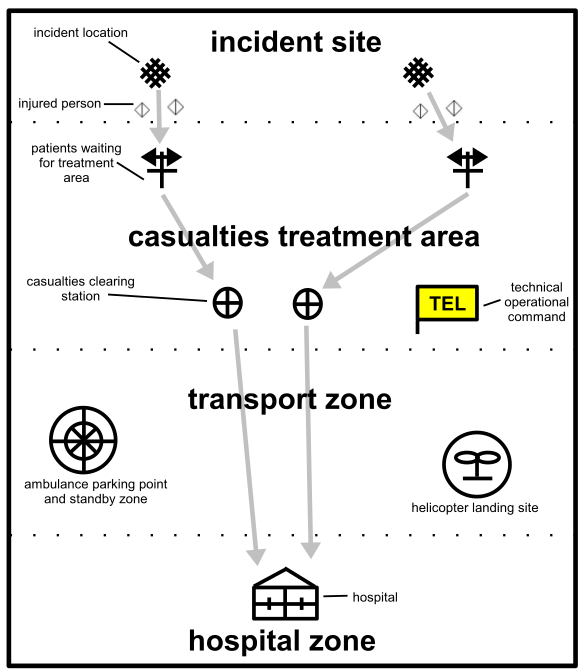
\includegraphics[width=280px]{disaster.png}
    \caption{Representación del escenario de desastre}
    \label{fig:disaster}
\end{figure}


Se define formalmente un escenario de desastre $S$ como un área de simulación dividida en áreas tácticas disjuntas: la zona del incidente (IL), zona de pacientes esperando tratamiento (PWT), estación de rescate de víctimas (CCS), punto de estacionamiento de ambulancias (APP), y un centro técnico operacional (TOC). La simulación coonsiste en un área $F$, un conjunto de áreas tácticas $R$, y un conjunto de obstáculos $H$. Un área táctica $r \in R$ es una tupla definida como

$$ r = (l_r, P_r, e_r, a_r, N_r^{stat}, V_r^{stat}, T_r^{stat}, G_r^{stat}, N_r^{trans}, V_r^{trans}, T_r^{trans}, G_r^{trans}, Z_r^{trans})$$

donde
\begin{enumerate}
\item $l_r \in \{IL, PWT, CCS, APP, TOC\}$ es la clasificación del área táctica,
\item $P_r \subset F$ es una parte poligonal del área F,
\item $e_r$ y $a_r$ son dos puntos al borde de $P_r$, de entrada y salida respectivamente,
\item $N_r^{trans}$ y $N_r^{stat}$ son dos conjuntos de nodos
\item $V_r^{trans}$ y $V_r^{stat}$ son los intervalos de velocidad $[v_{min}, v_{max}]$de los nodos en $N_r^{trans}$ y $N_r^{stat}$,
\item $N_r^{trans}$ y $N_r^{stat}$ son los intervalos de tiempo $[t_{min}, t_{max}]$ para las pausas de los nodos en $N_r^{trans}$ y $N_r^{stat}$,
\item $N_r^{trans}$ y $N_r^{stat}$ son los tamaños de los grupos de nodos en $N_r^{trans}$ y $N_r^{stat}$,,
\item $Z_r$ es la secuencia de puntos o ciclo de movimiento de los nodos de transporte.

\end{enumerate}

Cada área táctica $r$ tiene un punto de entrada $e_r$ y un punto de salida $a_r$. Los nodos que transportan pacientes pueden dejar las áreas sólo mediante estos puntos. Este modelo es motivado por los puntos de registro de entrada y salida para los pacientes. Cada nodo es asignado a un área táctica, pudiendo ser \emph{estacionario}, es decir, permanece dentro de su área táctica y sólo se mueve dentro de $P_r$; o es un nodo de transporte, acarreando pacientes entre distintas áreas basado en el movimiento dado por $Z_r$. Los nodos estacionarios se denominan $N_r^{stat}$, mientras que los de transporte se denominan $N_r^{trans}$. 


\subsection{Definición de las zonas}

Para los centros técnicos operacionales y estaciones de rescate, se asume que los nodos son todos estacionarios, es decir,

$$\forall r \in R| l_r \in \{CSS, TOC\} : N_r^{trans} = \emptyset, Z_r^{trans} = \emptyset$$

Por otra parte, las zonas de incidentes consiste exclusivamente de nodos de transporte, es decir,

$$\forall r \in R| l_r \in \{IL\}: N_r^{stat} = \emptyset$$

Los nodos de transporte $n \in N_r^{trans}$ de la locación de incidentes comienzan en el punto $a_r$. Allí selecciona un punto aleatorio $rand \in P_r$ y se mueve a ese punto. Desde allí se mueve hasta el punto de salida $a_r$ y se mueve hacia un punto aleatorio de la zona \emph{pacientes esperando tratamiento}, $e_{PWT_{rand}}$. Finalmente, se mueve de vuelta al punto $a_r$. Este ciclo modela el recoger a un paciente de la zona de incidentes y llevarlo a la zona de tratamientos. En los puntos $rand$ y $e_{PWT_{rand}}$ se realiza una pausa de acuerdo a una distribución uniforme tomada de $T_r^{trans}$. Con esto se modela la primera asistencia a los pacientes 


\textbf{Pacientes esperando tratamiento:} $r \in R | l_r = PWT$
Se realiza un ciclo entre $PWT$ y $CCS$ o estación de rescate de víctimas. 

\textbf{Estacionamiento de ambulancias:} $r \in R | l_r = APP$
Los nodos de transporte se mueven tras entrar al escenario por la entrada $e_r$, a un punto aleatorio $rand \in P_r$ dentro del área. Después de una pausa de un tiempo aleatorio, se abandona el estacionamiento usando el punto $a_r$. Desde ahí, se mueven a la salida $a_r$, desde donde se mueven a una salida $a_{CSS_{rand}}$ de una estación de rescate de víctimas (CSS) aleatoria. Realizan otra pausa en este lugar, y luego abandonan el escenario.
Este movimiento describe ambulancias que entran, se estacionan, recogen a pacientes para llevarlos al hospital y abandonan el escenario. 

\subsection{Manejo de obstáculos}

Se considera la zona de simulación $F$ como planar y estática, con un conjunto de obstáculos poligonales simples (sin hoyos ni autointersecciones) $H$. Se utilizan métodos de planificación de movimiento de robots para decidir las rutas. Se asume que las áreas tácticas $P_r$ son también polígonos simples.

Para encontrar el mejor camino, se utilizan grafos de visibilidad. Esto es, un grafo donde sus vértices son los vértices de los obstáculos, y existe un arco entre dos vértices si se puede "ver", es decir, no intersecta el interior de ningún obstáculo. Se añaden las entradas y salidas de las zonas como vértices al grafo. Luego de calcular el grafo, se asignan pesos según la distancia euclidiana. Con esto, se puede utilizar el algoritmo de Dijkstra para encontrar el conjunto de arcos que componen el mejor camino.

\newpage
\end{comment}

\section{Escenario de Mina Subterránea}

\subsection{Escenario}

\subsubsection{Descripción}

El escenario está compuesto por las siguientes zonas poligonales y adyacentes, cuya distribución se puede ver en la Figura \ref{fig:underground}. Por simplicidad, el dibujo se representa con rectángulos. Las áreas se conectan entre ellas con puntos de acceso específicos.

\begin{enumerate}
    \item \textbf{Centro Civico (CEC):} Es el área donde comienza la comunicación hacia el exterior, y el punto inicial y final de los operarios de la mina. Esta zona cuenta con conectividad total hacia el exterior, por lo que se puede considerar la zona final para la información.
    
    \item \textbf{Zona de Acceso (ACC):} El área de ingreso que conecta las zonas laterales y de extracción. Esta zona cuenta con conectividad hacia el centro cívico, pero con baja densidad de antenas.
    
    \item \textbf{Zona de extracción (EXT):} Es el área más relevante de la mina. No cuenta con conectividad. En esta zona se concentra el movimiento de los distintos nodos.
    Está conformado por una estructura de grilla que representan los posibles caminos dentro del área. Los ejes verticales están completamente despejados, mientras los ejes horizontales contienen obstáculos en el $70\%$ de los casos\footnote{Esto es una estimación muy arbitraria, ya que no pude conseguir un número }. En los bordes superior e inferior se ubican entre 1 y 4 DUMP, puntos de descarga, dependiendo del tamaño de la mina.
        
    \item \textbf{Zonas laterales(LAT):} Representan los accesos a los niveles superiores e inferiores de la mina donde ocurren otras operaciones, tal como la explotación en el nivel superior o el chancado primario en el nivel inferior. Por simplicidad topológica, las consideraremos áreas a los costados de la zona de Acceso.

    \item \textbf{Zona de mantención (MAN):} Representan los lugares donde se realiza mantención y actividades operativas, como carga de combustible. Estas zonas son aledañas a la zona de extracción EXT, y puede serlo a la zona de acceso ACC. En el escenario pueden existir 1 o 2 zonas de mantención, dependiendo del tamaño de la mina.
    
\end{enumerate}

\begin{figure}[H]
    \centering
    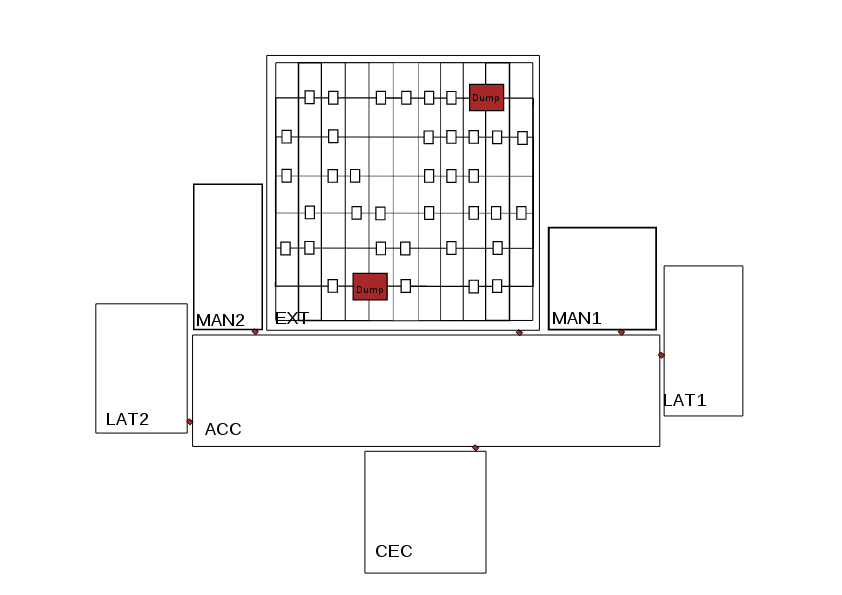
\includegraphics[width=400px]{underground2.png}
    \caption{Areas y conexiones del modelo de mina subterránea.}
    \label{fig:underground}
\end{figure}

\subsubsection{Restricciones}

Existen algunas restricciones que se imponen en el diseño de las distintas áreas que se listan a continuación.

\begin{itemize}

    \item El tamaño de la mina es una variable de la que dependerán las dimensiones de las distintas áreas, y en particular la zona de extracción, el número de DUMP y el número de áreas MAN. Además, el tamaño de la mina define el número de nodos dentro de ella. Se considerará un número entre 1 y 5, siendo 1 una mina pequeña y 5 una mina muy grande.
    
    \item La zona de extracción tiene exclusividad temporal para las LHDs, es decir, una vez trazada una ruta de la LHD, otras LHDs u operarios no pueden utizar esa ruta. 
    
    \item Existen interrupciones por explosión, que cierran y paralizan temporalmente la operación en un punto de intersección, sus 2 caminos aledaños verticales, y sus 2 aledaños horizontales. Estas pausas son breves y permiten continuar la operación normalmente. Su frecuencia tiene una distribución normal en torno a 1 cada 3 horas. 
    
\end{itemize}

\subsection{Movilidad}

\subsubsection{Tipos de Nodos}

\begin{enumerate}
    %personas
    
    \item Operarios (OP): Son los encargados del funcionamiento global. Son del tipo estático, trabajando en sólo una zona: MAN o CEC. Se mueven en grupos entre 1 y 3 personas, sólo dentro de
    
    \item Operarios de Mantenimiento (OM): Son los encargados de realizar actividades breves de mantenimiento en distintas zonas. Se mueven en grupos de entre 3 y 5 entre todas las áreas, realizando trabajos (pausas) en todas las zonas: CEC, ACC, EXT, LAT y MAN.
    
    \item Supervisores (SU): Son quienes supervisan las actividades. Son entre 1 y 2, y recorren las distintas áreas de manera pseudoaleatoria siguiendo decisiones representadas como una cadena de Markov\footnote{El motivo de usar una cadena de Markov para supervisores, es que un ciclo sería demasiado determinista, pero aleatorio sería irreal; una cadena de markov permite un buen orden con alta probabilidad, pero permite incorporar casos distintos que son frecuentes. Esto es totalmente arbitrario de lo que me han comentado 2 supervisores de cómo es, definitivamente necesita validación.}, como se ve en la Figura \ref{fig:markov}
    
    %maquinas
    
    \item Camionetas (CA): Son equivalentes a los operarios de mantención, pero a una velocidad mayor y se desplazan individualmente. 
    
    \item Load, Haul, Dump Machines (LHD): Son las máquinas de carga, recorrido y descarga. Su movimiento se restringe a las zonas EXT y MAN. Su movimiento sigue el siguiente algoritmo\footnote{Mi propuesta es que se use una distribución de Poisson para la pausa de las máquinas, ya que es canónica para modelar en torno a un promedio los sucesos raros: en nuestro caso, que una mantención resulte ser una falla que requiere más tiempo de pausa.}:
    \end{enumerate}
    \begin{verbatim}
definir DUMP de la LHD
for(random 50-200):
    seleccionar punto aleatorio P en el área EXT no reservada.
    for(random 10-30):
        ir a P. pausa aleatoria ~15s
        recorrer mejor ruta sin obstáculos para llegar a DUMP. v=12km/h
        ir a DUMP. pausa aleatoria ~5s
    end
    ir a la zona de mantención más cercana, a través de la zona de $ACC$. 
    Pausa en torno a 30m según distribución de Poisson
end
\end{verbatim}

\begin{enumerate}
  \setcounter{enumi}{5}
    \item Martillos picadores (MP): Son estáticos y se ubican en sobre los puntos de DUMP. Dada su operación remota, se considera que son puntos de acceso a la red \emph{backbone} cableada.
\end{enumerate}


\begin{figure}
\begin{center}
\begin{tikzpicture}[->, >=stealth', auto, semithick, node distance=9cm]
\tikzstyle{every state}=[fill=white,draw=black,thick,text=black,scale=0.8]
    \node[state]    (A)                     {CEC};
    \node[state]    (B)[right of=A]   {ACC};
    \node[state]    (C)[below right of=A]   {EXT};
    \node[state]    (D)[above of=B]   {LAT$_i$};
    \node[state]    (E)[below right of= B]  {MAN$_m$};
\path

%centro civico
(A) edge[loop left]             node{$0.6$}                                 (A) %me quedo en CC
    edge[bend left]             node{$0.4$}                                 (B) %ir al área de decision
    
%acceso    
(B)
    edge[bend left]             node{$0.3$}                                 (A) %volver al CC
    edge[bend right, left]      node{$0.3$}                                 (C) %ir al area de extraccion
    edge[bend left, left]       node{$\frac{0.2}{|M|}, \forall m \in M$}    (D) %ir a laterales
    edge[bend left, right]      node{$\frac{0.2}{|I|}, \forall i\in I$}     (E) %ir a una de las mantenciones
    
%extraccion
(C) edge[loop right]            node{$0.2$}                                 (C) %ir a otro punto en el área de extracción
    edge[bend right, right]     node{$0.2$}                                 (B) %volver al al acceso
    edge[bend left, above]      node{$0.2$}                                 (A) %volver al CC
    
%laterales
(D) edge[bend left, right]      node{$0.3$}                                 (B) %volver al acceso
    edge[bend right, above] node{$0.7$}                                 (A) %volver al CC
    
%mantencion
(E) edge[loop right]            node{$\frac{0.4}{|I|}, j\neq i, j\in I$}    (E) %ir a otra mantención
    edge[bend left]            node{$0.3$}                                  (B) %volver a la zona de extracción
    edge[bend left=70]             node{$0.3$}                                 (A);%volver al CC

\end{tikzpicture}
\caption{Autómata representando transiciones para los supervisores}
\label{fig:markov}
\end{center}
\end{figure}

\newpage
\section{Definición Formal}

Formalmente, definiremos un escenario de minería subterránea como un área de simulación dividida en áreas disjuntas, de los tipos $CEC, ACC, EXT, LAT$ y $MAN$, representando las zonas previamente definidas. Las áreas $CEC, ACC$ y $EXT$ son únicas, $LAT$ son dos, y $MAN$ pueden ser 1 o 2 dependiendo del tamaño de la mina.

A diferencia del escenario de desastre, los nodos no pertenecen a un área táctica única, sino que su tipo determina su patrón de movilidad, donde todos comienzan desde el área $CEC$, exceptuando las $LHD$.
La simulación coonsiste en un área $F$, un conjunto de áreas tácticas $R$, y un conjunto de obstáculos $H$. Un área táctica $r \in R$ es una tupla definida como

$$ r = (l_r, P_r, A_r, D_r, C_r, R(t))$$

donde
\begin{enumerate}
\item $l_r \in \{CEC, ACC, EXT, LAT, MAN\}$ es la clasificación del área táctica,
\item $P_r \subset F$ es una parte poligonal del área F,
\item $A_r$ es el conjunto de puntos $a_r$ de acceso, situados al borde de $P_r$.
\item $C_r$ es el conjunto de obstáculos.
\item $D_r$ es un conjunto de obstáculos que determinan una zona de atracción para los distintos nodos.
\item $R_r(t)$ es un conjunto de obstáculos dependientes del tiempo generados por las restricciones de acceso en las distintas zonas por los nodos.
\end{enumerate}
Por su parte, los nodos y sus patrones de movilidad están definidos como:

$$ n = (t_n, d_n, V_n^{ml}, V_n^{Ml}, Z_r) $$

donde
\begin{enumerate}
\item $t_n \in \{OP, OM, SU, CA, LHD. MP\}$ es la clasificación del tipo de nodo
\item $V_n^{ml_r}$ y $V_n^{Ml_r}$ son los intervalos de velocidad $[v_{min}, v_{max}]$ para el nodo en un área del tipo $l_r$.
\item $N_n$ es el tamaño de los grupos de nodos.
\item $Z_n^{l_r}$ es el ciclo de movimiento del nodo dentro de un área de tipo $l_r$.

\end{enumerate}

\end{document}